% !TEX root = deplump.tex
\newcommand{\T}{\ensuremath{\mathcal{T}}}
\newcommand{\N}{\ensuremath{\mathcal{N}}}
\newcommand{\M}{\ensuremath{\mathcal{M}}}
\newcommand{\PP}{\ensuremath{\mathcal{P}}}
\newcommand{\nc}{\ensuremath{nc}}
\newcommand{\RS}{\ensuremath{\mathcal{R}\mathcal{S}}}
\newcommand{\D}{\ensuremath{\mathcal{D}}}

\begin{figure*}[t] 
	\begin{center}
		\scalebox{.6}{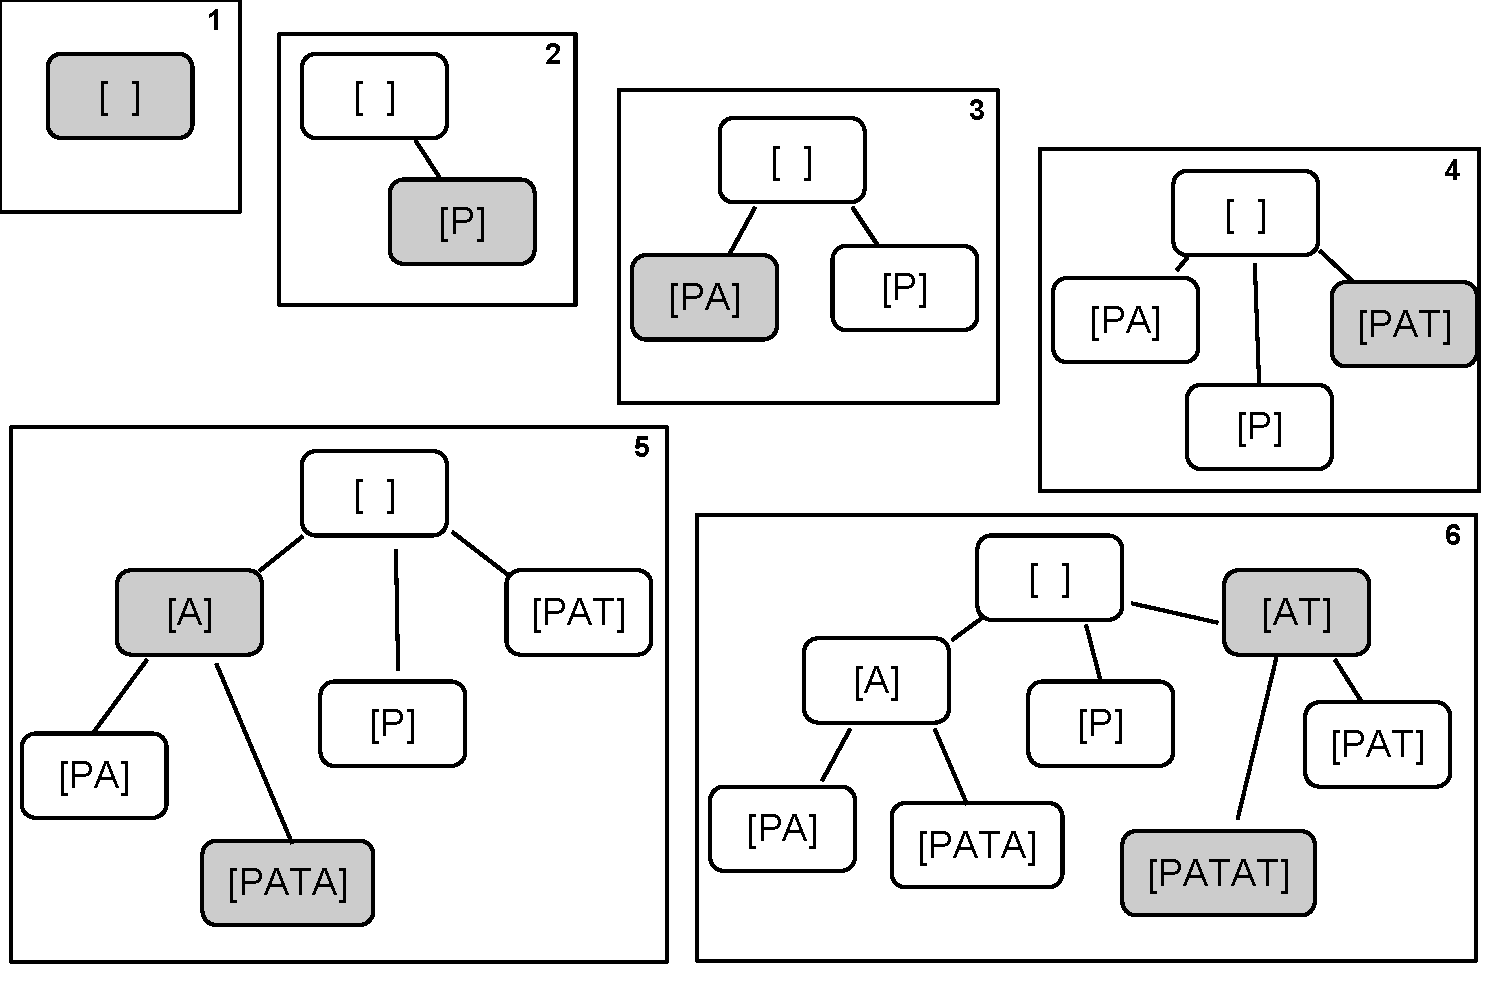
\includegraphics{PATAT.pdf}} % [clip=true, viewport= 1in 1in 9in 9in]
		\caption{Construction of suffix tree for string ``PATAT".  In each frame the new nodes are shaded in gray.}
		\label{fig:suffix_tree}
	\end{center} 
\end{figure*} 

Probabilistic compression algorithms work by using a generative model to predict the sequence.  The predictive distribution function is then used as the parameter in a range encoder to compress the stream.  The details of a range encoder implementation are not included here, we only note that if the predictive distribution function is $F$ and the next symbol in the stream is $s$ then the parameters required by the range encoder are $F(s-1)$ and $F(s)$.  In order to decompress the stream the exact same predictive model will need to be built.  This requires that the model estimate prior to compressing $s_n$ is a function of fixed parameters and the symbols $[s_0, s_1, \ldots, s_{n-1}]$ because those are the only symbols available to the decompressor for decompressing $s_n$.  

The algorithm operates primarily on a suffix tree.  A suffix tree is a data structure for keeping track of unique suffices of a set of strings.  The tree structure arranges the suffices hierarchically which makes it easy to search.  In the case of single stream the set of strings to consider is the set of contexts $\{ [ ], [s_0], [s_0,s_1], [s_0, s_1,s_2], \ldots \}$.  The suffix tree is comprised of nodes, each corresponding to a context of the form $[s_m, \ldots, s_{m + k}]$.  Nodes other than the root have exactly one parent, but could have many children.  

The suffix tree must be incrementally constructed as elements of the sequence are processed.  Construction of the tree is handled by the function GetNode in Algorithm~\ref{alg}.  An illustration of the incremental suffix tree construction can be seen in Figure~\ref{fig:suffix_tree} for the toy sequence [PATAT].  Note that in frame 5 the node [A] had to be inserted in order to incorporate the node [PATA].  Using the notation of GetNode([PATA], \T) to describe the frame we find \N \space = [PATA], \M \space = [PA],  and \PP\space = [A].

\begin{algorithm}
    \caption{Deplump} \label{alg}
    \begin{algorithmic}[1]
    
    	\Procedure{Deplump}{{\bf s } = $[s_0, s_1, s_2, \ldots , s_m]$, depth}
		\State Set \nc \space = 0 (node count), \RS \space = [ ] (reference sequence)
		\State Initialize \T \space (tree) and update \nc
		\State Set \D \space $= \{ d_0, d_1, d_2, \dots, d_{\min(10,depth)}, \alpha \}$ (discount parameters)
		\For{i = 0 : m}
			\State [$F(s-1), F(s)$] = CDFNextSymbol($s_i$,\T,\RS)
			\State Update discount parameters based on gradients and learning rate
			\State Use range encoder to encode the symbol $s_i$ using values of $F(s-1)$ and  $F(s)$
			\State Add $s_i$ to \RS
		\EndFor
	\EndProcedure
	
    	\Function{CDFNextSymbol}{$s$,\T,\RS}	
		\While{\RS \space is longer than allowable}
			\State Shorten reference sequence
		\EndWhile
		\While{ \nc \space $>$ (max allowable nodes - 2)}
			\State Delete leaf node uniformly at random
		\EndWhile
		
		\State \N =  GetNode(\RS, \T)
		\State [$F(s-1), F(s)$] = CDF($s$, \N, cdf = zero array, $d$ = 1)
		\State UpdateCountsAndDiscounts(\N,$s$, TRUE)
		\State \Return [$F(s-1), F(s)$]
	\EndFunction
	
	\Function{GetNode}{Context, \T}
		\State \N \space is a node/context corresponding to \RS
		\State Find the node \M \space in suffix tree sharing the longest suffix with \N
		\If{\M \space is a suffix of \RS}
			\If{\N \space is not equal to \M}
				\State Add node \N \space as a child of \M
				\State \Return \N
			\Else
				\State \Return \M
			\EndIf
		\Else
			\State \PP \space = GetNode(shared suffix of \M \space and \N, \T)
			\State Add node \N as a child of \PP \space for the current context
			\State \Return \N
		\EndIf
	\EndFunction
	 \end{algorithmic}
\end{algorithm}

\begin{algorithm}
    \caption{Deplump Continued}
    \begin{algorithmic}[1]
    
    	\Function{UpdateCountsAndDiscounts}{\N, $s$, AddCount}
		\If{AddCount}
			\State $c^\N_s += 1$
			\State AddCount = 1 with probability $\frac{t^\N d^\N}{c^\N_s + (t^\N - t^\N_s)d}$ else 0 
			\State $t^N_s += ({\rm AddCount} == 1)$
		\EndIf
		\State Update discount parameter gradients
		\State UpdateCountsAndDiscounts(parent of \N, $s$, AddCount)
	\EndFunction	


	\Function{CDF}{$s$, \N, cdf, $m$}
		\For{i = 1 : size of symbol set }
			\State cdf[i] += $m(\frac{c^\N_i - t^\N_i d^\N}{c^\N})$
		\EndFor
		\If{\N \space has parent}
			\State \Return CDF($s$, parent of \N, cdf, $d^\N m$)
		\Else
			\State cdf = (1- $d^\N m$)cdf + $d^\N m$(uniform distribution over symbol set) 
			\State $F(s-1)$ = sum(cdf(1:($s$-1)))
			\State \Return [$F(s-1), F(s) = F(s-1)$ + cdf($s$)]
		\EndIf 
	\EndFunction
    \end{algorithmic}
\end{algorithm}

\begin{algorithm}
	\begin{algorithmic}[1]
	\caption{Creating the Tree}
	
	\Function{FractureNode}{$\N,d,c$}
		\State Initialize \M (a new node)
		\For{each $s$ observed in node \N}
			\State partition = GetPartition($c^\N_s, t^\N_s$,-c)
			\State Set $c^\M_s = 0$, $t^\M_s = t_s$, and $t_s = 0$
			\For{$i$ = 1 : length(partition)}
				\State Set t = DrawCRP(partition[i],d,c)
				\State Set $t^\N_s, c^\M_s += t$
			\EndFor
		\EndFor
	\EndFunction
	
	\Function{GetPartition}{$c,t,d$}
		\State Set $M =  d \times$ $c$ matrix of zeros
		\State Set $M(d,c) = 1.0$
		\For{$j = (c-1) : 1$}
			\For{$i = 1 : (t-1)$} 
				\State Set $M(i,j) = M(i +1, j+1)(id)  + M(i+1,j)(j - id)$ 
			\EndFor
			\State Set $M(d,j) = M(t,j+1)$
		\EndFor
		\State Set partition = $[p_1, p_2, \ldots, p_t]$ with $p_i = 0$ for $i >1$ and $p_1 = 1$
		\State Set $k = 1$
		\For{j = 2 : c}
			\State Set $M(k,j) = M(k,j)(j-1 -k d)$
			\State Set $M(k+1,j) = M(k+1,j)kd$
			\State Set $r = 1$ with probability $\frac{M(k+1,j)}{M(k+1,j) + M(k,j)}$ else 0
			\If{r == 1}
				\State $k += 1$
				\State partition[$k$] = 1
			\Else
				\State partition$[m] += 1$ with probability $\frac{{\rm partition}[m] - d}{j-1 -kd}$ for $1 \leq m \leq k$
			\EndIf
		\EndFor
		\State \Return partition
	\EndFunction
	
	\Function{DrawCRP}{$n,d,c$}
		\State Set $t = 1$
		\For{i = 2 : n}
			\State Set $r = 1$ with probability $\frac{td + c}{i-1 + c}$ else 0
			\State Set $t += (r == 1)$
		\EndFor
		\State \Return $t$
	\EndFunction
	
	\end{algorithmic}	
\end{algorithm}